% For submission to GPS hello
\documentclass[gpscopy,onehalfspacing,11pt]{ubcdiss}


%% NFSS font specification (New Font Selection Scheme)
\usepackage{times,mathptmx,courier}
\usepackage[scaled=.92]{helvet}

%% Math or theory people may want to include the handy AMS macros
\usepackage{amssymb}
\usepackage{amsmath}
\usepackage{amsfonts}
\usepackage{enumitem}
\usepackage{pdflscape}



\usepackage{pifont}
\usepackage{multirow}

\usepackage{nicefrac}

% https://stackoverflow.com/questions/1673942/latex-table-positioning
\usepackage{float}
\restylefloat{table}



%%%%%%%%%%%%%%%%%%%%%%%%%%%%%%%%%%%%%%%%%%%%%%%%%%%%%%%%%%%%%%%%%%%%%%

\usepackage[table]{xcolor}
\usepackage{multicol}
\usepackage{threeparttable}

%%%%%%%%%%%%%%%%%%%%%%%%%%%%%%%%%%%%%%%%%%%%%%%%%%%%%%%%%%%%%%%%%%%%%%
\usepackage{checkend}	% better error messages on left-open environments

\usepackage[pdftex]{graphicx} % for incorporating external images
% declare the path(s) where your graphic files are
\graphicspath{ {./fig/} }
% % and their extensions so you won't have to specify these with
% % every instance of \includegraphics
\DeclareGraphicsExtensions{.png,PNG,.pdf,.jpg,.jpeg}


%% booktabs: provides some special commands for typesetting tables as used
%% in excellent journals.  Ignore the examples in the Lamport book!
\usepackage{booktabs}

\usepackage{listings}
\lstset{basicstyle=\sffamily\scriptsize,showstringspaces=false,fontadjust}

%% The acronym package provides support for defining acronyms, providing
\usepackage[printonlyused,nohyperlinks]{acronym}
\renewcommand{\acsfont}[1]{{\scshape \MakeTextLowercase{#1}}}

\usepackage{color}
\definecolor{greytext}{gray}{0.5}
\definecolor{lightgray}{gray}{0.9}

\usepackage{comment}

\usepackage[numbers,sort&compress]{natbib}
\newcommand{\citeeg}[1]{\citep[e.g.,][]{#1}}

%% The titlesec package provides commands to vary how chapter and
\usepackage[compact]{titlesec}
\titleformat*{\section}{\singlespacing\raggedright\bfseries\Large}
\titleformat*{\subsection}{\singlespacing\raggedright\bfseries\large}
\titleformat*{\subsubsection}{\singlespacing\raggedright\bfseries}
\titleformat*{\paragraph}{\singlespacing\raggedright\itshape}

%% The caption package provides support for varying how table and
\usepackage[format=hang,indention=-1cm,labelfont={bf},margin=1em]{caption}

%% url: for typesetting URLs and smart(er) hyphenation.
%% \url{http://...} 
\usepackage{url}
\urlstyle{sf}	% typeset urls in sans-serif


%%%%%%%%%%%%%%%%%%%%%%%%%%%%%%%%%%%%%%%%%%%%%%%%%%%%%%%%%%%%%%%%%%%%%%
%% Other possibly useful packages

\usepackage{soul}
\usepackage{lipsum}
\usepackage[framemethod=tikz]{mdframed}
\usepackage{hanging}
% \usepackage{tikz}


% https://tex.stackexchange.com/questions/172475/how-can-i-define-a-custom-tcolorbox-environment-with-color-as-a-parameter
% https://tex.stackexchange.com/questions/66154/how-to-construct-a-coloured-box-with-rounded-corners
\usepackage{tcolorbox}
% \newtcolorbox{rndbox}{colback=red!5!white,colframe=red!75!black}

\newtcolorbox{rndbox}[1]{coltitle=black,colframe=blackcolor,fonttitle=\bfseries,title=#1}
%  https://tex.stackexchange.com/questions/19646/how-to-typeset-special-apple-mac-keyboard-symbols
\usepackage{menukeys}

% https://tex.stackexchange.com/questions/316334/after-clearpage-move-the-figure-to-the-top
\usepackage{afterpage}

\usepackage[bookmarks,bookmarksnumbered,%
    allbordercolors={0.8 0.8 0.8},%
    pagebackref,linktocpage%
    ]{hyperref}

    
%% The following change how the the back-references text is typeset in a
\newcommand{\nocitations}{\relax}

\renewcommand*{\backrefsep}{,~}%
\renewcommand*{\backreftwosep}{,~}% ', and~'
\renewcommand*{\backreflastsep}{,~}% ' and~'
\renewcommand*{\backrefalt}[4]{%
\textcolor{greytext}{\ifcase #1%
\nocitations%
\or
\(\rightarrow\) page #2%
\else
\(\rightarrow\) pages #2%
\fi}}


%% The following uses most defaults, which causes hyperlinks to be
% \usepackage[bookmarks,bookmarksnumbered]{hyperref}

% \usepackage[bookmarks,bookmarksnumbered,pdfborder={0 0 0}]{hyperref}

%% The following disables all hyperlinking, but still enabled use of
%% \autoref{}
%\usepackage[draft]{hyperref}

%% The following commands causes chapter and section references to
%% uppercase the part name.
\renewcommand{\chapterautorefname}{Chapter}
\renewcommand{\sectionautorefname}{Section}
\renewcommand{\subsectionautorefname}{Section}
\renewcommand{\subsubsectionautorefname}{Section}

%%%%%%%%%%%%%%%%%%%%%%%%%%%%%%%%%%%%%%%%%%%%%%%%%%%%%%%%%%%%%%%%%%%%%%
%% Some special settings that controls how text is typeset
%%
% \raggedbottom		% pages don't have to line up nicely on the last line
% \sloppy		% be a bit more relaxed in inter-word spacing
% \clubpenalty=10000	% try harder to avoid orphans
% \widowpenalty=10000	% try harder to avoid widows
% \tolerance=1000

%% And include some of our own useful macros
% This file provides examples of some useful macros for typesetting
% dissertations.  None of the macros defined here are necessary beyond
% for the template documentation, so feel free to change, remove, and add
% your own definitions.
%
% We recommend that you define macros to separate the semantics
% of the things you write from how they are presented.  For example,
% you'll see definitions below for a macro \file{}: by using
% \file{} consistently in the text, we can change how filenames
% are typeset simply by changing the definition of \file{} in
% this file.
% 
%% The following is a directive for TeXShop to indicate the main file
%%!TEX root = diss.tex

\newcommand{\NA}{\textsc{n/a}}	% for "not applicable"
\newcommand{\eg}{e.g.,\ }	% proper form of examples (\eg a, b, c)
\newcommand{\ie}{i.e.,\ }	% proper form for that is (\ie a, b, c)
\newcommand{\etal}{\emph{et al}}

% Some useful macros for typesetting terms.
\newcommand{\file}[1]{\texttt{#1}}
\newcommand{\class}[1]{\texttt{#1}}
\newcommand{\latexpackage}[1]{\href{http://www.ctan.org/macros/latex/contrib/#1}{\texttt{#1}}}
\newcommand{\latexmiscpackage}[1]{\href{http://www.ctan.org/macros/latex/contrib/misc/#1.sty}{\texttt{#1}}}
\newcommand{\env}[1]{\texttt{#1}}
\newcommand{\BibTeX}{Bib\TeX}

% Define a command \doi{} to typeset a digital object identifier (DOI).
% Note: if the following definition raise an error, then you likely
% have an ancient version of url.sty.  Either find a more recent version
% (3.1 or later work fine) and simply copy it into this directory,  or
% comment out the following two lines and uncomment the third.
\DeclareUrlCommand\DOI{}
\newcommand{\doi}[1]{\href{http://dx.doi.org/#1}{\DOI{doi:#1}}}
%\newcommand{\doi}[1]{\href{http://dx.doi.org/#1}{doi:#1}}

% Useful macro to reference an online document with a hyperlink
% as well with the URL explicitly listed in a footnote
% #1: the URL
% #2: the anchoring text
\newcommand{\webref}[2]{\href{#1}{#2}\footnote{\url{#1}}}

% epigraph is a nice environment for typesetting quotations
\makeatletter
\newenvironment{epigraph}{%
	\begin{flushright}
	\begin{minipage}{\columnwidth-0.75in}
	\begin{flushright}
	\@ifundefined{singlespacing}{}{\singlespacing}%
    }{
	\end{flushright}
	\end{minipage}
	\end{flushright}}
\makeatother

% \FIXME{} is a useful macro for noting things needing to be changed.
% The following definition will also output a warning to the console
\newcommand{\FIXME}[1]{\typeout{**FIXME** #1}\textbf{[FIXME: #1]}}

% END

% Modified \textcircled solution
\newcommand*\circled[1]{\raisebox{.5pt}{\textcircled{\raisebox{-.9pt} {#1}}}}


% https://tex.stackexchange.com/questions/172475/how-can-i-define-a-custom-tcolorbox-environment-with-color-as-a-parameter
\definecolor{mycolor}{rgb}{0.122, 0.435, 0.698}
\definecolor{blackcolor}{rgb}{0, 0, 0}
\definecolor{lightgray}{gray}{0.9}

\definecolor{error}{HTML}{FFD5D4}
\definecolor{relevant}{HTML}{E0F8C7}
\definecolor{steelblue}{RGB}{0, 0, 152}
\definecolor{royalblue}{RGB}{65,105,225}
\definecolor{rufous}{rgb}{0.66, 0.11, 0.03}

\newmdenv[innerlinewidth=0.5pt, roundcorner=1pt,linecolor=blackcolor,innerleftmargin=4pt,
innerrightmargin=4pt,innertopmargin=4pt,innerbottommargin=4pt]{mybox}



% Author's comments
\newcommand{\gm}[1]{\textcolor{orange}{{\textit{GM: #1}}}}
\newcommand{\gcm}[1]{\textcolor{orange}{{\textit{GM: #1}}}}
\newcommand{\art}[1]{\textcolor{steelblue}{{\textit{AM: #1}}}}


% Bullet while on draft mode
\newcommand{\blt}{\smallskip \textbullet ~}


% Counters
\newcounter{rq}

\newcommand{\RQ}[1]{\textit{RQ\the\numexpr\arabic{rq}\relax}}


\newcommand{\red}[1]{\textcolor{red}{#1}}
\newcommand{\rev}[1]{\textcolor{steelblue}{#1}}
\newcommand{\orange}[1]{\textcolor{orange}{#1}}


\definecolor{Brow}{HTML}{792500}


% Highlight package, default colour set to ligthgray
\sethlcolor{lightgray}

% https://tex.stackexchange.com/questions/50792/a-better-pm-symbol
\makeatletter
\newcommand{\mypm}{\mathbin{\mathpalette\@mypm\relax}}
\newcommand{\@mypm}[2]{\ooalign{%
  \raisebox{.1\height}{$#1+$}\cr
  \smash{\raisebox{-.6\height}{$#1-$}}\cr}}
\makeatother


% https://tex.stackexchange.com/questions/22798/nice-looking-empty-set
\let\oldemptyset\emptyset
\let\emptyset\varnothing

\usepackage{pifont}% http://ctan.org/pkg/pifont
\newcommand{\cmark}{\ding{51}}%
\newcommand{\xmark}{\ding{55}}%

\newtcolorbox{bluequote}{enhanced,
  boxrule=0pt,
  frame hidden,
  borderline west={4pt}{0pt}{lightgray},
  colback=white,
  sharp corners,
  right=0pt, 
  top=0pt, 
  bottom=0pt}


% https://tex.stackexchange.com/questions/69148/how-to-insert-title-in-mdframed
\newenvironment{frameEnv}[1]
  {\mdfsetup{
    frametitle={\colorbox{white}{\space#1\space}},
    frametitlefont=\ttfamily,
	  innertopmargin=1pt,
    frametitleaboveskip=-\ht\strutbox,
    frametitlealignment=\center
    }
  \begin{mdframed}%
  }
  {\end{mdframed}}


\newtcolorbox{keyobs}[1][]{
  breakable,  
  colback=white,
  colbacktitle=white,
  coltitle=black,
  fonttitle=\bfseries,
  bottomrule=0pt,
  toprule=0pt,
  leftrule=3pt,
  rightrule=0pt,
  titlerule=0pt,
  arc=0pt,
  outer arc=0pt,
  colframe=black,
}



\newcommand{\boldparagraph}[2]{%
  \medskip%
  \begin{hangparas}{.0in}{0}%
    \textbf{#1} #2%
  \end{hangparas}%
}%





% example of minipage

% \begin{figure}
%   \centering
%   \begin{minipage}{.5\textwidth}
%       \centering
%       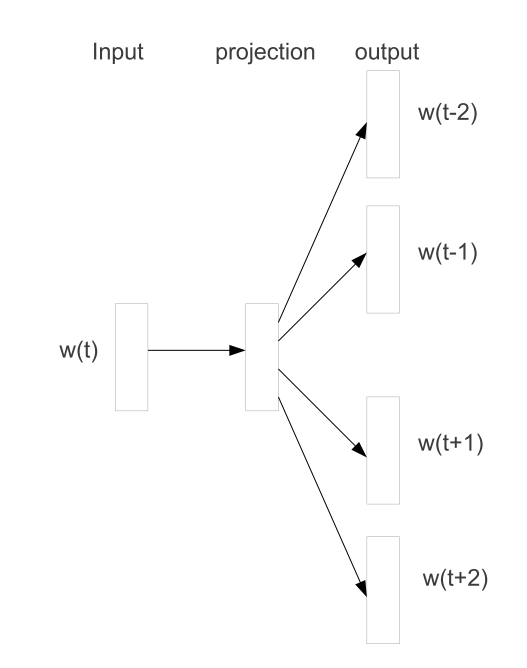
\includegraphics[width=0.5\linewidth, height=0.2\textheight]{fig/cp5/skip-gram-architecture}
%       \caption{The Skip-gram model architecture~\cite{Mikolov2013}}
%       \label{fig:skip-gram}
%   \end{minipage}%
%   \begin{minipage}{0.5\textwidth}
%       \centering
%       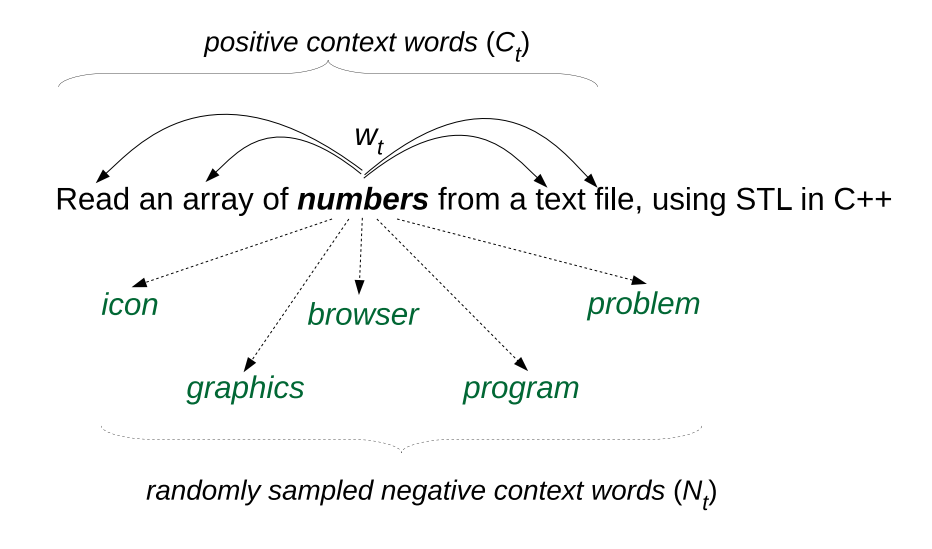
\includegraphics[width=\linewidth, height=0.2\textheight]{fig/cp5/ye-skip-gram-example}
%       \caption{Positive and negative training examples~\cite{Ye2016}}
%       \label{fig:skip-gram-example}
%   \end{minipage}
% \end{figure}



%%%%%%%%%%%%%%%%%%%%%%%%%%%%%%%%%%%%%%%%%%%%%%%%%%%%%%%%%%%%%%%%%%%%%%

\title{Supporting a Developer's Discovery \\ of Task-Relevant Information}
%\subtitle{If you want a subtitle}

\author{Arthur de Sousa Marques}
\previousdegree{B. Computer Science, Universidade Federal de Campina Grande, 2013}
\previousdegree{M. Computer Science,  Universidade Federal de Campina Grande, 2014}

% What is this dissertation for?
\degreetitle{Doctor of Philosophy}

\institution{The University of British Columbia}
\campus{Vancouver}

\faculty{The Faculty of Science}
\department{Computer Science}
\submissionmonth{August}
\submissionyear{2022}

% details of your examining committee
\examiningcommittee{Gail C. Murphy}{Supervisor}
\examiningcommittee{Muhammad Abdul-Mageed}{Supervisory Committee Member}
\examiningcommittee{Reid Holmes}{Supervisory Committee Member}
\examiningcommittee{Magnus Monolith, Other Department}{Additional Examiner} % TODO

% details of your supervisory committee
\supervisorycommittee{Reid Holmes}{Supervisory Committee Member}
\supervisorycommittee{Muhammad Abdul-Mageed}{Supervisory Committee Member}

%% hyperref package provides support for embedding meta-data in .PDF
%% files
\hypersetup{
  pdftitle={ (DRAFT: \today)},
  pdfauthor={Arthur Marques},
  pdfkeywords={Your keywords here}
}

%%%%%%%%%%%%%%%%%%%%%%%%%%%%%%%%%%%%%%%%%%%%%%%%%%%%%%%%%%%%%%%%%%%%%%

\begin{document}

% TODO uncomment
% \maketitle

% \makecommitteepage

% 

\chapter*{Abstract}

The information that a developer seeks to aid in the completion of a task typically exists across different kinds of software artifacts that include substantial natural language text. For instance,
artifacts vary from conversational discussions about bug reports to tutorial descriptions of features in a library.
In the artifacts that a developer consults, only some portions of the text will be useful to a developer's task
and locating such portions can be time-consuming as the artifacts can include substantial text to peruse organized in different ways. For example, it might be easier to locate information
in tutorial artifacts with structured headings whereas artifacts consisting of developer conversations might need to be read in detail. 
% \\

Given the limited time developers have to spend on any task, researchers have 
attempted to aid the developers by proposing a range of techniques to automate the identification of relevant text. 
However, this prior work is generally constrained to one or only a few types of artifacts.  
Enabling a developer access to artifact-specific approaches is difficult to deploy
and support to the multitude of artifact types that is constantly evolving
is challenging, if not impractical.
% \\

In this dissertation, we propose a set of generalizable techniques to aid developers in locating a portion of text that might be useful for a task. These techniques are based on semantic patterns that arise from the empirical analysis of the text relevant to a task in multiple kinds of artifacts, leading us to propose techniques that incorporate the semantics of words and sentences to identify text likely relevant to a developer's task automatically.
We evaluate the proposed techniques assessing the extent to which they identify text that developers deem relevant in different kinds of artifacts associated with Android development tasks. We then investigate how a tool that embeds the most promising semantic-based technique might assist developers while they perform a task. Results show that semantic-based techniques perform equivalently well across multiple artifact types and that a tool that automates the provision of task-relevant text assists developers in effectively completing a software development task.
    


% \cleardoublepage

% %% The following is a directive for TeXShop to indicate the main file
%%!TEX root = diss.tex

%% https://www.grad.ubc.ca/current-students/dissertation-thesis-preparation/preliminary-pages
%% 
%% LAY SUMMARY Effective May 2017, all theses and dissertations must
%% include a lay summary.  The lay or public summary explains the key
%% goals and contributions of the research/scholarly work in terms that
%% can be understood by the general public. It must not exceed 150
%% words in length.

\chapter{Lay Summary}

A software developer usually relies on web pages to find information that helps them complete a software task. 
However, only portions of the text in these web pages might be helpful to the developer's current task.
Finding the relevant parts can be difficult and require much time. The approaches that help developers perform this activity are limited to certain types of web pages, such as community forums, tutorials, and others. 
This thesis explores how we can find information relevant to a developer's tasks in a more general manner. 
First, we study text that developers find relevant to a task. 
Then we propose techniques that find such text automatically. 
We report how a tool built using one of these techniques helps developers perform a task. 
Results show that developers find that the text  identified automatically by the tool has helpful information that assists them in completing a software task.

% \cleardoublepage

% %% The following is a directive for TeXShop to indicate the main file
%%!TEX root = diss.tex

\chapter{Preface}

All of the work presented in this thesis was conducted in the Software Practices
Lab at the University of British Columbia, Point Grey campus.
Parts of the research presented in this dissertation has been previously published in the following articles:


% \begin{small}
\begin{enumerate}
    \item  Arthur Marques, ``\textit{Helping developers search and locate task-relevant information in natural language documents}'', 27th ACM Joint Meeting on European Software Engineering Conference and Symposium on the Foundations of Software Engineering (ESEC/FSE), 2019, pp. 1168-1171, doi: 10.1145/3338906.3341459
    \item  Arthur Marques, Nick C. Bradley and Gail C. Murphy, ``\textit{Characterizing Task-Relevant Information in Natural Language Software Artifacts}'', IEEE International Conference on Software Maintenance and Evolution (ICSME), 2020, pp. 476-487, doi: 10.1109/ICSME46990.2020.00052.
    \item  Arthur Marques, Giovanni Viviani and Gail C. Murphy, ``\textit{Assessing Semantic Frames to Support Program Comprehension Activities}'',  IEEE/ACM 29th International Conference on Program Comprehension (ICPC), 2021, pp. 13-24, doi: 10.1109/ICPC52881.2021.00011.
    \item   Arthur Marques and Gail C. Murphy, ``\textit{Evaluating the Use of Semantics for Identifying Task-relevant Textual Information}'',  2022 IEEE International Conference on Software Analysis, Evolution and Reengineering (SANER), 2022, pp. 240-251, doi: 10.1109/SANER53432.2022.00039
\end{enumerate}
% \end{small}




Part of this work involved other collaborators. Nick C. Bradley contributed in
the interview analysis described in Chapter~\ref{ch:characterizing}.
Alison Li, Katharine Kerr, and Tarc{\'i}sio Teixeira helped 
in the creation of the dataset presented in Chapter~\ref{ch:android-corpus}.
Giovanni Viviani helped in the analysis, design and implementation of the 
semantic parser used in Chapter~\ref{ch:identifying}.
Shaunak Tulshibagwale helped implementing some of the 
data gathering scripts for the 
corpora presented in Chapters~\ref{ch:identifying} and~\ref{ch:assisting}, respectively.
The scripts that gathered data from Stack Overflow are an extension of 
 Nadi and Treude's scripts~\cite{nadi2019Rep}.
Muhammad Abdul-Mageed was a supervisory committee member and helped providing access to the 
Compute Canada research grid used in the design and evaluation of the
approaches described in  Chapter~\ref{ch:identifying}.
Gail C. Murphy was the supervisory author on this project
and was involved throughout the project in concept formation, data analysis, and
manuscript composition.




All projects and associated methods were approved by the University of British Columbia's Research
Ethics Board [certificates \#H18-02104 and \#H19-04054].



% \cleardoublepage

% \tableofcontents
% \cleardoublepage	% required by tocloft package

% \listoftables
% \cleardoublepage	% required by tocloft package

% \listoffigures
% \cleardoublepage	% required by tocloft package

%% The following is a directive for TeXShop to indicate the main file
%%!TEX root = diss.tex

\chapter{Glossary}

This glossary uses the handy \latexpackage{acroynym} package to automatically
maintain the glossary.  It uses the package's \texttt{printonlyused}
option to include only those acronyms explicitly referenced in the
\LaTeX\ source.  To change how the acronyms are rendered, change the
\verb+\acsfont+ definition in \verb+diss.tex+.

% use \acrodef to define an acronym, but no listing
\acrodef{UI}{user interface}
\acrodef{UBC}{University of British Columbia}

% The acronym environment will typeset only those acronyms that were
% *actually used* in the course of the document
\begin{acronym}[ANOVA]
\acro{ANOVA}[ANOVA]{Analysis of Variance\acroextra{, a set of
  statistical techniques to identify sources of variability between groups}}
\acro{API}{application programming interface}
\acro{CTAN}{\acroextra{The }Common \TeX\ Archive Network}
\acro{DOI}{Document Object Identifier\acroextra{ (see
    \url{http://doi.org})}}
\acro{GPS}[GPS]{Graduate and Postdoctoral Studies}
\acro{PDF}{Portable Document Format}
\acro{RCS}[RCS]{Revision control system\acroextra{, a software
    tool for tracking changes to a set of files}}
\acro{TLX}[TLX]{Task Load Index\acroextra{, an instrument for gauging
  the subjective mental workload experienced by a human in performing
  a task}}
\acro{UML}{Unified Modelling Language\acroextra{, a visual language
    for modelling the structure of software artefacts}}
\acro{URL}{Unique Resource Locator\acroextra{, used to describe a
    means for obtaining some resource on the world wide web}}
\acro{W3C}[W3C]{\acroextra{the }World Wide Web Consortium\acroextra{,
    the standards body for web technologies}}
\acro{XML}{Extensible Markup Language}
\end{acronym}

% You can also use \newacro{}{} to only define acronyms
% but without explictly creating a glossary
% 
% \newacro{ANOVA}[ANOVA]{Analysis of Variance\acroextra{, a set of
%   statistical techniques to identify sources of variability between groups.}}
% \newacro{API}[API]{application programming interface}
% \newacro{GOMS}[GOMS]{Goals, Operators, Methods, and Selection\acroextra{,
%   a framework for usability analysis.}}
% \newacro{TLX}[TLX]{Task Load Index\acroextra{, an instrument for gauging
%   the subjective mental workload experienced by a human in performing
%   a task.}}
% \newacro{UI}[UI]{user interface}
% \newacro{UML}[UML]{Unified Modelling Language}
% \newacro{W3C}[W3C]{World Wide Web Consortium}
% \newacro{XML}[XML]{Extensible Markup Language}
	% always input, since other macros may rely on it

% \textspacing		% begin one-half or double spacing

% %% The following is a directive for TeXShop to indicate the main file
%%!TEX root = diss.tex

\chapter{Acknowledgments}



I cannot express how much I am grateful for my supervisor, Gail Murphy. I feel incredibly privileged to have been supervised by someone so respectful, attentive, and inspiring. Thank you. 

I am equally grateful for all the support my family and my partner, Lisley Siqueira, provided me over the last six years. Moving to an entirely new country and starting our life together was a rollercoaster, yet it was a journey full of love, empathy and self-discovery. 

I am thankful to my supervisory committee, Reid Holmes and Muhammad Abdul-Mageed, for all their support and feedback over the last years. Their curiosity encouraged me to explore and learn many new things. I am also thankful to the members of my examining committee, Luanne Sinnamon, Alexander Summers, and Christina von Flach, for their time and effort in reading my thesis and providing insightful feedback. 

I am indebted to many of the friends and colleagues I made at the University of British Columbia, the Software Practices Lab, the Library Research Commons, the Oakridge Adventist Church, and the Vancouver DnD Collective. Many thanks to old-time friends who kept in touch despite being spread across the globe. I cannot name all of you, but I want to thank you all.


Thanks to all the Computer Science Department staff and Elise Vredenbregt for helping with hectic calendars. I would also like to acknowledge the Natural Sciences and Engineering Research Council of Canada for supporting this work. 


\begin{flushright}
Arthur Marques

October 2022
\end{flushright}


\clearpage

\thispagestyle{empty}
\vspace*{\fill}
\begin{flushright}
\emph{To my partner, Lisley Siqueira}
\end{flushright}
\vspace*{\fill}




\clearpage
\thispagestyle{empty}
\vspace*{\fill}

\begin{flushright}
    \emph{Hoje longe, muitas l\'egua}

    \emph{Numa triste solid\~ao}

    \emph{Espero a chuva cair de novo}

    \emph{Pra mim vortar' pro meu sert\~ao}

    --- Asa Branca, song by Luiz Gonzaga
\end{flushright}
\vspace*{\fill}

\clearpage

%%%%%%%%%%%%%%%%%%%%%%%%%%%%%%%%%%%%%%%%%%%%%%%%%%%%%%%%%%%%%%%%%%%%%%

% Body of Thesis (not all sections may apply)
\mainmatter

\acresetall	% reset all acronyms used so far


\setcounter{chapter}{3}
\setcounter{rq}{1}


\chapter{Identifying Task-Relevant Text}
\label{ch:identifying}


\stepcounter{rq}

\vspace{1mm}

\begin{enumerate}[label=\textit{RQ\arabic*},leftmargin=1.4cm]
\setcounter{enumi}{\the\numexpr \arabic{rq} - 1\relax}

\item \textit{What techniques can we use to automatically extract text relevant to a software developer's task?} 

\end{enumerate}

\vspace{1mm}

--- Chapter introduction 

------ Use findings of characterization studies (cp3) to motivate the need for the techniques proposed in this chapter

------ Brief summary of techniques we propose

------ Brief summary of evaluation and results



\clearpage


\section{Approach}
\textcolor{white}{force ident} % this is just for the chapter outline

--- We address the problem of automatically detecting task-relevant text in a \textit{artifact-agnostic} way. \vspace{3mm}

--- To design our approaches, we use the manually curated task-relevant sentences produced in our characterization study~\cite{marques2020} \vspace{3mm}

--- We investigate two main approaches:

------ \textit{Heuristic-based}: uses a set of properties in the text (including \textit{semantic frames}~\cite{fillmore1976frame}) to determine if a given sentence is relevant to the input task

------ \textit{ML-based}: uses the novel \textit{Transformer}~\cite{Vaswani2017attention} neural network to jointly model the relevancy of a given input sentence with respect to a task. 

--- Explain why we have selected these two approaches

------ With our first approach, we investigate whether a light-weight technique addresses the need of automatically identifying task-relevant text, what could potentially discourage the need for more complex and computationally expensive solutions~\cite{Bavota2016}

------ Our second approach investigates the applicability of pre-trained models that do not require large amounts of training data to our domain problem~\cite{devlin2018bert, Ye2016}. With this approach, we revisit findings on the trade-offs of using machine learning techniques to mine textual data~\cite{Chaparro2017, Bavota2016}.



\clearpage

\section{Task-pertinent Artifacts Corpus}
\textcolor{white}{force ident} % this is just for the chapter outline

--- To evaluate the techniques proposed in this chapter, we require a sufficiently large corpus containing 
software tasks and associated artifacts originating from heterogeneous sources.
Unfortunately, such a corpus is not promptly available and thus, 
this section outlines the steps we took for its creation.


\section{Software Tasks}
\textcolor{white}{force ident} % this is just for the chapter outline

--- We consider a software task as a piece of work undertaken by a developer that often has to be finished within a certain time~\cite{2004merriam}. 
Two common places a software task can be found are:

\begin{itemize}
    \item the description of a bug or feature request reported in a bug tracking systems; or in
    \item a post in a community forum, development mailing lists, and others.
\end{itemize}

\vspace{3mm}

--- Given this definition, we select tasks from StackOverflow and GitHub to build our corpus

------ We scope task selection to the \textit{Android} development domain such that we can select common tasks across the two sources \vspace{3mm}



--- Detail that StackOverflow tasks were selected from Baltes et al. dataset~\cite{baltes2019-rep}

------ Give example of a StackOverflow task \vspace{5mm}

--- Because there is no GitHub dataset promptly available, we selected GitHub issues from top starred Android projects on GitHub 

------ Projects were selected among Open Source Systems that had the \textit{Java} and \textit{Android} tags. 

------ We randomly sampled 15 issues from a total of 10 distinct projects

------ Describe how we avoid common pitfalls  when mining GitHub~\cite{kalliamvakou2014}

------ Give example of a GitHub task 

\section{Artifact Selection}
\label{cp4:corpus-artifacts}
\textcolor{white}{force ident} % this is just for the chapter outline


--- Our artifact selection approach seeks to simulate everyday practices on how developers search the Web~\cite{rao2020, Xia2017} \vspace{3mm}

--- To that end, we consider a task's title (i.e., SO question or GitHub issue title) as the seed used to search for pertinent artifacts in a search engine

------ This is a common procedure adopted by many studies in the field (e.g.,~\cite{Xu2017} or ~\cite{Silva2019}). \vspace{3mm}


--- As there are many different sources of artifacts, we restrict artifact selection to well known and studied sources~\cite{Starke2009,Kevic2014, Li2013}:


\begin{itemize}
    \item Android and Java SE API documentation;
    \item Github issues;
    \item StackOverflow answers; and
    \item Websites from the java and android categories on Alexa~\cite{alexa}.
\end{itemize}


\vspace{3mm}

--- For these sources, we use the \texttt{googlesearch} API~\cite{googlesearch} to perform Web searches

------ Results were limited to English and a maximum of 5 resources per source 

------ These limitations were necessary because of throttling or even blocking mechanisms in the APIs used the fetch data in each of the sources considered \vspace{3mm}

--- Provide descriptive statistics for the corpus

------ 300 tasks, 150 from SO and 150 from Git

------ Approximately 2,500 artifacts

------ Almost 260,000 sentences

\clearpage


\section{Analytic Evaluation}
\textcolor{white}{force ident} % this is just for the chapter outline

--- To be able to judge the accuracy of any technique used to automatically identify sentences relevant to a task,
we require test data comprising sentences that contain information needed for task completion. \vspace{3mm}

--- We rely on human experts to produce this data \vspace{3mm}


--- With the experts data, we report a technique's accuracy for the given task and artifact source

------ For sources that have been evaluated in other studies, i.e., API documentation~\cite{Robillard2015}, GitHub issues~\cite{Lotufo2012}, and StackOverflow answers~\cite{Xu2017}, we compare the accuracy of our techniques 
to the state-of-the-art

------ To show that our techniques extend beyond well known/studied sources, we also report our techniques accuracy on miscellaneous sources, e.g., Websites from Alexa



\subsection{Golden Standard}
\textcolor{white}{force ident} % this is just for the chapter outline

--- Creating test data for the entirety of our corpus is infeasible so we restrict our evaluation to a subset of 10 tasks evenly sampled from the two types of tasks in the corpus (i.e., 5 GitHub tasks and 5 StackOverflow tasks) \vspace{3mm}

--- For these tasks, golden data consists of any sentence that two or more experts have deemed as useful for task-completion \vspace{3mm}



\subsubsection{Annotators}
\textcolor{white}{force ident} % this is just for the chapter outline

--- We recruited \red{n} graduate students with professional programming experience to produce \textit{golden} data for these 10 tasks. \vspace{3mm}


\subsubsection{Annotation Procedures}
\textcolor{white}{force ident} % this is just for the chapter outline

--- Our intention is that goldens reflect text that an \textit{expert} would deem as useful for task completion. \vspace{3mm}


--- To produce such data, annotators had a set of randomly assigned tasks description and links to artifacts 
pertinent to the respective task at their disposal \vspace{3mm}

--- We asked annotators to write a short comment (250 words max~\cite{Rastkar2010}) with instructions that a newcomer could follow to successfully complete the task.

------ The purpose of the comment was to ensure that annotators built enough context about the task \vspace{3mm}

--- Once the comment was written,  annotators had to manually highlight sentences that they deemed useful and that provide information that assists task completion.

--- Three different individuals performed each task. \vspace{3mm}

--- An in-house tool in the form of a Web browser plugin facilitated annotation procedures

\subsection{Method}
\textcolor{white}{force ident} % this is just for the chapter outline

--- For each task, we have a set of artifacts with sentences identified by experts that contain information relevant to the task \vspace{3mm}

--- For each task and artifact type, we apply the appropriate technique (baseline and ours) to automatically detect task-relevant text in that artifact

--- We then compute the technique's accuracy against the experts' highlights 

--- We use the obtained values to discuss the accuracy of each technique on their respective artifacts



\subsubsection{Baselines}
\label{cp4:comparison-techniques}
\textcolor{white}{force ident} % this is just for the chapter outline

--- We systematically reviewed related work and we identified techniques applicable to our domain problem

------ Selection criteria considered each technique's availability in existing replication packages and their readiness for use.

------ We also refrained from using approaches with training procedures (e.g., ~\cite{liu2020} or ~\cite{Treude2016}) because of ~\cite{Chaparro2017, fucci2019} \vspace{3mm}


--- Based on these criteria, we selected the following techniques for comparison:


\begin{itemize}[leftmargin=\parindent, font=\normalfont\itshape]
    \item \textit{SO Answers} (\texttt{AnsBot})~\cite{Xu2017} --- short description of the approach;
    
    \item \textit{API Documentation} (\texttt{APIRef})~\cite{Robillard2015} --- short description of the approach;
    
    \item \textit{GitHub issues} (\texttt{HurriedBug})~\cite{Lotufo2012} --- short description of the approach;

    \item \textit{Miscellaneous} (\texttt{LexRank})~\cite{Erkan2004} --- in the lack of an artifact-specific technique for this category, we use LexRank as a baseline because it has been evaluated in several studies that address the identification of textual information in natural language software artifacts~\cite{nadi2020, Ponzanelli2017}
\end{itemize}






\subsubsection{Evaluation Metrics}
\textcolor{white}{force ident} % this is just for the chapter outline

--- We use the golden data to compute precision and recall


--- For a given task $t$ and artifact $a$, precision is computed as the ratio between the sentences identified that are indeed relevant (i.e., sentences identified by the experts) and the total number of sentences identified by the technique


\begin{equation}
    Precision(t, a) = \frac{\# \text{\textit{sentences identified that were marked as relevant by the experts}}}{\# \text{\textit{sentences identified}}}
\end{equation}

\vspace{3mm}

--- Recall represents how many relevant sentences are identified by a technique


\begin{equation}
    Recall(t, a) = \frac{\# \text{\textit{sentences identified that were marked as relevant by the experts}}}{\# \text{\textit{sentences marked as relevant by the experts}}}
\end{equation}

\vspace{3mm}

--- When comparing techniques, we favor precision instead of recall because false positives may contribute to a developer abandoning reading of an artifact that would otherwise provide crucial information for her task~\cite{Rastkar2010}.


\subsection{Results}
\textcolor{white}{force ident} % this is just for the chapter outline

--- Discuss results \vspace{3mm}

\subsection{Threats to Validity}

--- Discuss threats \vspace{3mm}

\clearpage


\section{Human Evaluation}
\textcolor{white}{force ident} % this is just for the chapter outline

\red{argument to justify this second evaluation}

--- Although our analytic evaluation gives insight on how accurately can we identify text relevant to a task within a natural language artifact, we seek to provide further evidence on whether software developers consider automatically detected text as useful for a task 

--- In this study, we asked software developers to indicate if automatically detected text provided important/useful information needed to correctly accomplish a task.

--- This evaluation was performed on a random sample of 30 tasks in our corpus (distinct from the expert tasks)

--- To avoid confirmation biases, developers provided input for both text detected by one of our approaches (i.e., the approach that had the best results in our analytic evaluation) and text detected by approaches in the literature (Section~\ref{cp4:comparison-techniques})



\subsection{Participants}
\textcolor{white}{force ident} % this is just for the chapter outline

--- For this evaluation, we consider the challenges of recruiting software developers in the local area and we instead opt to use 
\textit{Amazon Mechanical Turk}~\cite{mturk} (MTurk).

--- Background questions ensured that individuals had Java development experience and that they had familiarity with the artifact sources in our corpus.

--- Specifically, a MTurk evaluator---\textit{turker}--- had to answer the following background questions:


\begin{enumerate}[leftmargin=\parindent, font=\normalfont\itshape, label=BQ\textsubscript{\arabic*.}]
    \item Is developing software part of your job? Yes, no 
    \item For how many years have you been developing software? Free text
    \item How would you rate your development expertise in Java? No experience at all developing Java, Beginner, Intermediate, Expert
    \item How would you rate your development expertise in Android? No experience at all developing Android, Beginner, Intermediate, Expert
    \item When performing a software task, what sources do you normally seek information on? Multiple choice: API documentation, Stack Overflow, Github, Medium, ...
\end{enumerate}

   

\subsection{Method}
\textcolor{white}{force ident} % this is just for the chapter outline


--- All the evaluation was performed in the Mechanical Turk platform. \vspace{3mm}

--- Turkers indicated the relevancy of a sentence to a given task  by answering the question: \vspace{3mm}

\begin{enumerate}[leftmargin=\parindent, font=\normalfont\itshape, label=SR\textsubscript{\arabic*}]
    \item Which of the following statements best describes this sentence? 
    \textit{(a)} The sentence is meaningful and provides important/useful information needed to correctly accomplish the task in question, 
    \textit{(b)} The sentence is meaningful, but does not provide any important/useful information to correctly accomplish the task in question, 
    \textit{(c)} The sentence does not make sense to me.
\end{enumerate}

--- We deliberately word the question as close as possible to other peer-reviewed studies in the field~\cite{nadi2020, Xu2017}. \vspace{3mm}


--- Due to constraints on the platform, the evaluators judged sentences individually, i.e., without access to the context in which the sentences appeared. \vspace{3mm}

--- Turkers also had to answer a \textit{quality-gate task} randomly drawn from the experts' tasks.

------ The task showed five expert-curated sentences (all marked by the experts as relevant) and a turker had to indicate the sentences' usefulness as in any other task.

------ We discarded responses from any turker who deemed less than three out of the five sentences as useful for the task


\subsubsection{Evaluation Metrics}
\textcolor{white}{force ident} % this is just for the chapter outline

--- We report a quantitative analysis of the ratings provided by the turkers




\subsection{Results}
\textcolor{white}{force ident} % this is just for the chapter outline

--- Discuss results \vspace{3mm}

\subsection{Threats to Validity}

--- Discuss threats \vspace{3mm}

\clearpage

\section{Summary}
\textcolor{white}{force ident} % this is just for the chapter outline

--- Summary of contributions for the chapter \vspace{3mm}

------ A corpus containing 300 software tasks originating from StackOverflow and Github and associated artifacts containing potentially relevant information to correctly completing the task \vspace{3mm}

------ Two artifact-agnostic techniques for automatically detecting text relevant to an input task in a given artifact

------ Empirical comparison of our techniques to existing techniques in the literature

------ Study with human evaluators on whether they consider automatically detected text as useful for task completion


\setcounter{chapter}{4}
\setcounter{rq}{1}


\chapter{Identifying Task-Relevant Text}
\label{ch:identifying}

The information a developer seeks to help aid the completion of a task typically exists
across a range of artifacts. 
To aid developers identify, from the large amount of text
in these documents, just the fraction of text relevant
to the task-at-hand, prior work has used syntactic properties of the text
---alongside an artifact's meta-data---
 to identify likely relevant text (\red{Chapter~\ref{}}).
Although effective, these techniques target specific
types of artifacts, limiting their use across the 
many different kinds of artifacts developers encounter
daily in their work.



In this chapter, we explore a design space of possible techniques building on approaches to interpret the meaning, or semantics, of text
to identify task-relevant text across different kinds of software artifacts.
We introduce six possible techniques that incorporate the  
semantics of words and sentences. 
We show that some of the proposed semantic-based techniques 
compare to existing artifact-specific techniques 
and that they apply to a broader set of artifacts.






%To answer this question, we explore a set of approaches from previous related work and of our own 
%for the automatic identification of text that might contain information relevant to a particular software task.
%Through usage of human-annotated data produced earlier in this thesis, we 
%investigate how accurately can these techniques identify text relevant to software development task.
We start by outlining the hypotheses that motivate the techniques that we explore (Section~\ref{cp5:motivation}) followed by detailed descriptions of the
techniques (Section~\ref{cp5:approaches}).
We show how the six techniques 
compare against state-of-the-art artifact-specific techniques and 
their accuracy across different types of artifacts (Section~\ref{cp5:evaluation}). 
Section~\ref{cp5:summary} summarizes our key findings.

\clearpage




% 
\section{Problem Statement}
\label{cp5:motivation}





Researchers have long recognized the value of natural language
text, utilizing various approaches to extract
information from this text that can be embedded in
tools for software developers \red{ref}.
These approaches exploit lexical and semantic properties available in the text to determine 
whether it contains information of interest to a developer \red{ref}. 
In this work, information of interest represents text that a developer would consider as relevant to a specific software task. Ideally, we could establish that text in a natural language artifact that matches  
words (or terms) also present in a task description is likely relevant to the developer's task. However, direct matches are often scarce and researchers have observed that:



\medskip
\begin{bluequote}
    \textit{The text  that contains information associated with the solution for a task in a natural language artifact often differs from the text in the software task itself.}
\end{bluequote}
% \smallskip



Due to these differences, automatically determining the text in a natural language artifact that is of interest to a software task is not trivial. 
It requires techniques able to shorten the gap between the two sources, identifying or establishing relationships that would indicate the relevance of the text to the task-at-hand.


As a first step towards addressing this problem, we consider a set of techniques
 building on approaches to interpret the meaning, or semantics, of text.
 For that, we first provide theoretical background for the approaches that we explore. Then, we detail how we use these approaches in the design space of a technique that automatically identifies text relevant to a software task.







% \section{Approaches}
\label{cp5:approaches}

\gm{Perhaps you could consider a structure for this 
chapter that has: 1) Problem Definition (which is the 'all approaches
below' 2) Baseline 3) Approaches. The reason is to try to make
it clear what is a baseline and what are new proposed
approaches. Let's discuss.}

In this section, we detail three approaches to automatically identify text that is relevant to a particular software task.
These approaches encompass lexical similarity, word semantics, and frame semantics.


\gm{Argument below will need specific references back
to earlier chapters (eventually).}
All approaches take a task and a pertinent artifact as inputs and output the sentences 
that are most likely to contain information that assists a developer in completing their task. 
To determine how many sentences an approach should identify, we consider that 
no more than 20\% of the content in the artifacts in the
 \acs{DS-synthetic} and the \acs{DS-android} corpora are deemed relevant to a task, which, on average, accounts for 8.93 sentences
 and we approximate these values to identifying a target number of 10 sentences per input task-artifact. 
Our decision to output a certain number of sentences regardless of the approach is to have an easy framework for their comparison (Section~\ref{cp5:evaluation}).


\subsection{Lexical Similarity}

As a baseline, we investigate if the sentences that are lexical similar
to a task are more likely to contain information relevant to that task. \gm{Need argument why this is a good baseline.}


We use Vector Space Model (VSM)~\cite{Salton1975vsm} from Information Retrieval~\cite{Manning2009IR}
to compute the lexical similarity between the sentences within a pertinent artifact and a task. 
VSM represents both a task and individual sentences within an artifact as vectors of term weights,
where the weight of a term
can be computed using a Term-Frequency Inverse-Document-Frequency scheme (\textit{tf.idf})~\cite{Manning2009IR}. 
Once we obtain vector representations $t$ and $s$ 
for an input task and an arbitrary artifact sentence, 
their lexical similarity can be computed 
using the cosine similarity between their vectors, as Equation~\ref{eq:lex-sim} shows:



\begin{equation}
    cos(t,s) = \frac{t^Ts}{\|t\| \|s\|}
    \label{eq:lex-sim}
\end{equation}
\smallskip

By ranking the sentences in an artifact according to their similarity scores, i.e., from highest to lowest,
we can  select the top-n sentences as the ones relevant to an input task.

\gm{This section likely needs to provide a direct definition
of document in terms of artifacts.}

% ------------------------------------------------


\subsection{Word Semantics}


Language models capture (\gm{or represent or describe?}) the semantics of words based on the context in which words appear~\cite{harris1954distributional}.
They allow a more ``human-like reasoning'' even when words are lexically different, which 
motivates investigating whether we can identify task-relevant text by semantically matching the text in a pertinent artifact to the text in a task.



We first describe how we use language models to automatically identify task-relevant text, and then
detail how we use a baseline model \gm{I think this overloads
the word baseline} and 
a state-of-the-art model to automatically identify task-relevant text.
For an introduction of general concepts behind language models, please refer to~\cite{zhang2021deep-learning}.

\subsubsection{Background}

% introduce language models
A core concept of a language model is Harris' distributional hypothesis~\cite{harris1954distributional}, which states that words that appear in a similar context tend to have similar meanings.


A language model exploits this hypothesis by building vector representations, namely \textit{word embeddings}, for each of the words in a text corpus.
For that, it requires a significantly large number of sentences so that
the model associates similar vector embeddings to words that are similar in meaning~\cite{Ye2016}. 


% Overview of baseline model
\smallskip
\begin{hangparas}{.0in}{0}
     \textit{ Skip-gram model.} One common challenge to language models is that they need to learn word vector representations that are good at predicting the nearby words at low computational costs, e.g., the time needed to train a model, the model size, etc.
    The \textit{Skip-gram} model~\cite{Mikolov2013}, proposed by Mikolov et al., addresses such challenges using simple yet efficient training procedures. As Figure~\ref{fig:skip-gram-example} illustrates, the model learns vector representations by \textit{(i)} looking at the $n$ words that preceded and succeed word $w_t$
     as positive training examples, and by \textit{(ii)} randomly sampling words that do not appear in the same context as negative training examples. Empirical results have shown that negative sampling allows for an accurate model able to handle noise data and that 
     the vector representations provided by the model could be used to improve many natural language processing tasks~\cite{mikolov2013efficient}.
\end{hangparas}

\begin{figure}[H]
    \centering
    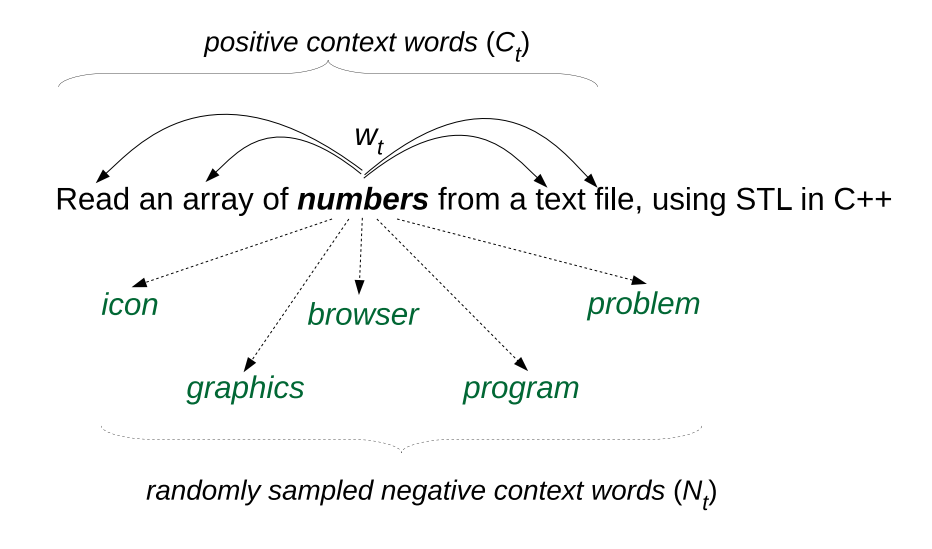
\includegraphics[width=.65\linewidth]{fig/cp5/ye-skip-gram-example}
    \caption{Positive and negative training examples in the Skip-gram model. Figure originally from~\cite{Ye2016} \gm{Unfortunately you can't use this diagram without permission if it is from a published text.}}
    \label{fig:skip-gram-example}
\end{figure}


Using the skip-gram model, one can identify that words $t$ and $s$ are semantically similar 
computing the cosine similarity between their corresponding word embedding representations, i.e., $w_t$ and $w_s$:



\begin{equation}
    cos(w_t,w_s) = \frac{w_t^Tw_s}{\|w_t\| \|w_s\|}
    \label{eq:word-sim}
\end{equation}




% Overview of state-of-the-art model
\medskip
\begin{hangparas}{.0in}{0}
     \textit{BERT model.} Context in the Skip-gram model refers to the positive/negative examples used during the model's training procedures; this, however, does not allow the model to disambiguate words based on their surrounding text. In other words, a Skip-gram model will have a single vector representation for the word \textit{company} even when it can have different meanings, i.e., a business organization or being with someone. In contrast, state-of-the-art models, such as \textit{BERT}~\cite{Devlin2018Bert}, provide different representations for the same word based on the sentence in which a word appears.
    This additional layer allows for more complex operations, such as word disambiguation \red{ref}.
\end{hangparas}



BERT also addresses tasks that need to understand relationships between sentences, which is a task not directly captured by language modeling~\cite{Devlin2018Bert}. \gm{I am struggling with the
idea that tasks 'need' to understand relationships between sentences. More explanation is likely needed.}
To capture sentence relationships, BERT training procedures consider both next word prediction---as in any language model---and also next sentence prediction, i.e., given a pair of sentences $A$ and $B$, the model 
is trained to predict the likelihood that sentence $B$ succeeds (or not) sentence $A$ (Figure~\ref{fig:BERT}). 


\begin{figure}
    \centering
    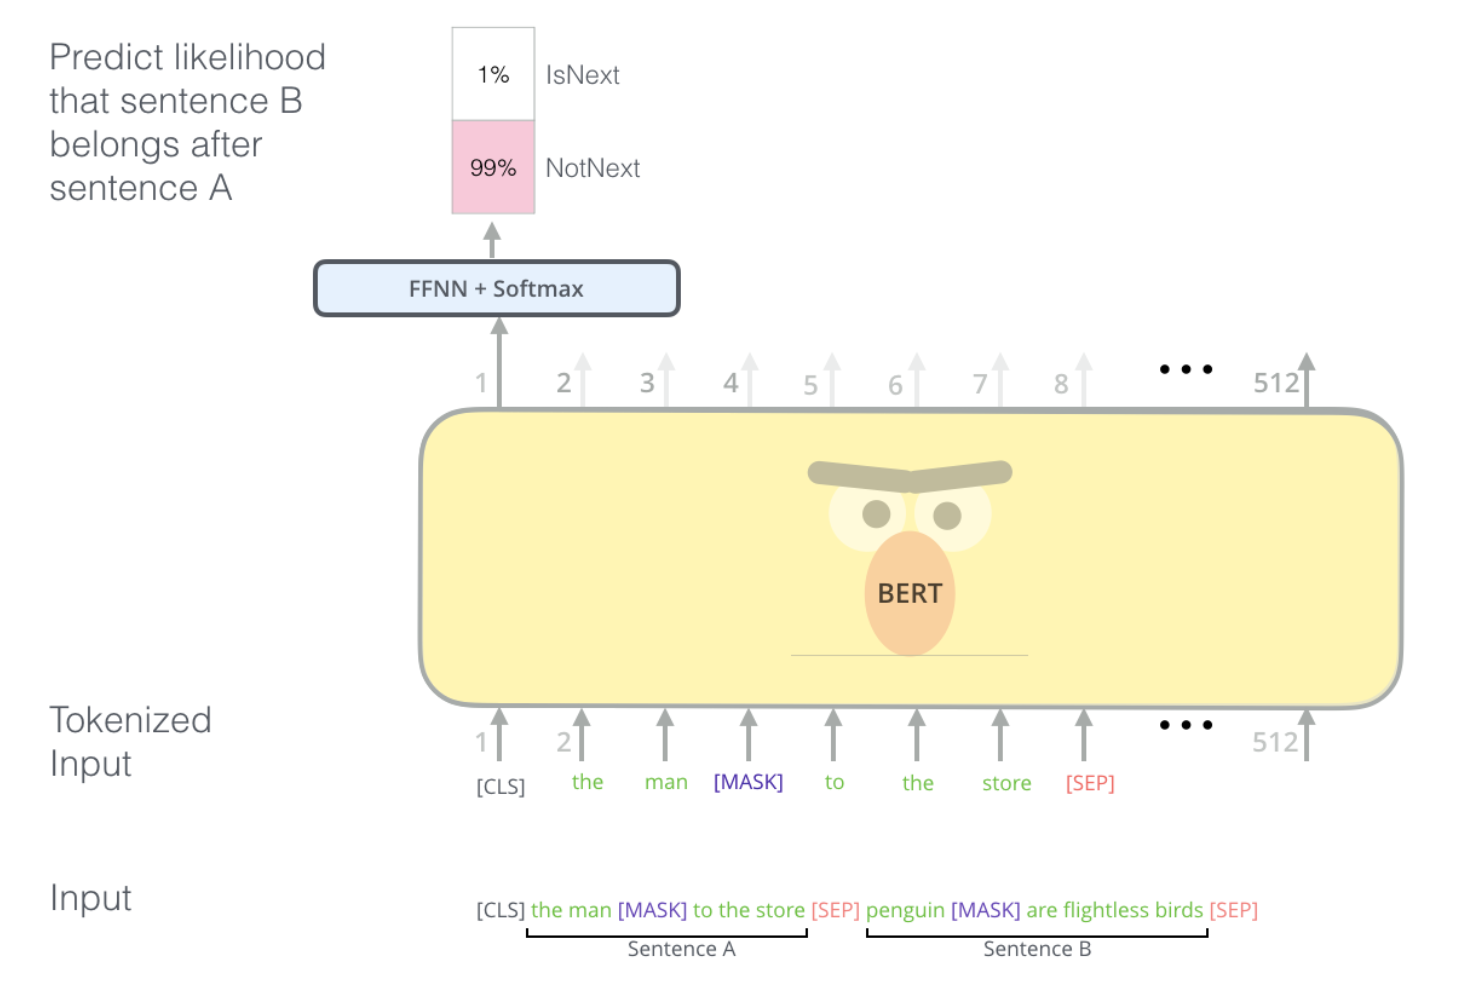
\includegraphics[width=.75\linewidth]{fig/cp5/BERT}
    \caption{BERT next sentence prediction training procedures. Figure originally from~\cite{jay-alammar-bert} \gm{Same issue
    with re-using Figure}}
    \label{fig:BERT}
\end{figure}



Since BERT addresses both next word prediction and next sentence prediction, the model can be used for several
word semantics and sentence relationship tasks such as  ours, i.e., determine the relevance of a sentence within an artifact based on a second sentence representing a task description. \gm{How is
this sentence prediction? Is there precendence for using
BERT on two different artifacts (i.e., the task description
can be considered an artifact or document.)}


% ------------------------------------------------


\subsubsection{Semantic Similarity}
\label{cp5:skip-gram}

\gm{Is this still part of background? There needs to be
some more walking the reader through where this part is
going. Maybe introduction some nomenclature for
actual approaches you are introducing. Let's discuss.}

Similar to lexical similarity,  we investigate if the sentences with the highest semantical similarity are most likely to contain information relevant to the input task.


To compute the semantic similarity between the sentences within a pertinent artifact and a task,
we use the Skip-gram model~\cite{Mikolov2013} with word embeddings specifically trained for the software engineering domain~\cite{Efstathiou2018}.
Since word embeddings provide vector representations at the word level, we follow Conneau et al.'s guidelines~\cite{conneau2018} 
and compute vector representations for an entire sentence by averaging the sum of the word embeddings in that sentence.


Provided that we have embeddings $w_t$ and $w_s$ for the text 
of an input task and an arbitrary artifact sentence, 
their semantic similarity can also be obtained 
using the cosine similarity. In turn, we can select the top-n sentences
with the highest semantical similarity as the ones likely relevant to an input software task.


% ------------------------------------------------


\subsubsection{Artifact-Task Sentence Relationships}
\label{cp5:bert}


We use the BERT model~\cite{Devlin2018Bert} to establish relationships between artifact and task sentences pairs and determine 
the sentences within an artifact that most likely contain information relevant to the task.


Since BERT requires training procedures, we start with an already pre-trained model, namely BERT\textsubscript{uncased}, and we tune it to  identifying task-relevant text.
\gm{Is BERT\textsubscript{uncased} something from elsewhere?}
As done by several other studies (e.g., ~\cite{Chaparro2017, fucci2019, Petrosyan2015}), we use standard cross-validation techniques to ensure  that no data used for evaluation is also used
during the model's training procedures. More specifically, we use 10-fold cross-validation with 70\%, 20\% and 10\% splits for training, validation and testing. 


The model outputs probability scores indicating the likelihood of a sentence being relevant to an input task.
We select the top-n sentences predicted by the model as relevant.



% ------------------------------------------------


\subsection{Frame Semantics}


\art{I still need to check frames based on the tasks in \acs{DS-synthetic}, so there might be updates to this section. }


Given our analysis of relevant sentences in the \acs{DS-synthetic} corpus, we pose that 
sentences with certain meanings, such as the ones that provide instructions on using an entity to achieve some goal,
are sentences that a developer would first pay attention to when inspecting a software artifact and thus, they are more likely to contain task-relevant information. \gm{Will need more on why
this hypothesis.}



We implement this hypothesis as a post-filtering step~\cite{Manning2009IR} applied to the lexical similarity and word semantics approaches.
Given a set of sentences returned by an approach, 
we use the \textit{SEFrame} tool~\cite{marques2021} as a proxy to the sentence's meaning,
checking if the semantic frames obtained by the tool appear in a set of frames drawn from  sentences annotated as relevant in the \acs{DS-synthetic} corpus.





% ------------------------------------------------


\subsection{Approaches Summary}


Table~\ref{tbl:approaches-summary} bundles the approaches that we explore.
The table provides a short identifier for each approach, identifies the research topic that serve as a basis for each approach and provides a short description for them. From now on, we refer to each approach according to their short identifier.

\gm{Isn't there multiple SEframes approaches?}


\begin{table}[H]
\centering    
\begin{scriptsize}
\begin{threeparttable}
\rowcolors{2}{}{lightgray}    
\begin{tabular}{lll}

% \hline

% \multicolumn{2}{c}{\textit{No lock screen controls ever}}  \\



\textbf{Identifier} & \textbf{Based on} & \textbf{Description} \\

\hline


\texttt{baseline} & 
\parbox[l][1cm][c] {1.5cm}{lexical\\similarity} &
\parbox[l][1cm][c] {8.5cm}{
    Uses VSM to identify the top-n sentences most lexically similar to a task description as task-relevant
}
\\


\texttt{word2vec} & 
\parbox[l][1cm][c] {1.5cm}{word\\semantics} &
\parbox[l][1cm][c] {8.5cm}{
    Uses the Skip-gram model to identify the top-n sentences most semantically similar to a task description as task-relevant
}
\\

\texttt{BERT} & 
\parbox[l][1cm][c] {1.5cm}{word\\semantics} &
\parbox[l][1.4cm][c] {8.5cm}{
    Uses BERT to establish relationships between a task description and sentences within an artifact, selecting the top-n sentences 
    that the model predicts as task-relevant
}
\\


\texttt{frame-meaning} & 
\parbox[l][1cm][c] {1.5cm}{frame\\semantics} &
\parbox[l][1cm][c] {8.5cm}{
    \red{TODO}
}
\\


\texttt{frame-matching} & 
\parbox[l][1cm][c] {1.5cm}{frame\\semantics} &
\parbox[l][1cm][c] {8.5cm}{
    \red{TODO}
}
\\



\hline


\end{tabular}
\end{threeparttable}
\end{scriptsize}
\caption{Summary of approaches used to automatically identify task-relevant text}
\label{tbl:approaches-summary}
\end{table}


% \clearpage

\section{Evaluation}
\label{cp5:evaluation}



The goal of our evaluation is to assist the design of tools that use the explored techniques to help developers in locating text relevant to their task. 
To evaluate and compare the techniques,
we report \textit{precision} and \textit{recall} metrics~\cite{manning2010IR} measuring what portion of the \acs{DS-android} text identified by human annotators the techniques automatically identify.
In this context, we believe recall to be the most important metric since failure to identify text that is relevant to a task means that a developer will have an incomplete or partial view of the information needed,
what can lead to faults~\cite{Murphy2005}.
Experimental procedures are as follows.



\subsubsection{Baseline}


As done by~\cite{Lin2021} and~\cite{Ye2016}, we use a standard \texttt{VSM} lexical similarity approach as a baseline. Our rationale to use 
lexical similarity as a baseline is based on the fact that 
both our qualitative analysis (\red{Chapter~\ref{aaa}}) and
related work~\cite{Ko2006a, Freund2015} have shown that developers often use keyword-matching as a first search strategy to locate text that might contain information relevant to their tasks.


Analogous to the semantic similarity-based technique (Section~\ref{cp5:approach-w2v}), the baseline technique uses VSM to compute lexical similarity scores. The baseline outputs the top-n sentences with the highest similarity as the ones likely relevant to an input software task.




\subsubsection{Setup}



We configure each technique to identify a target number of 10 relevant sentences per input task-artifact.
This decision is based on the fact that no more than 20\% of the content of any artifact in the corpora is deemed relevant to a task, which, on average, accounts for 8.93 sentences (\red{Chapter~\ref{}}).
Researchers have also used the same target number of 10 sentences when evaluating techniques  (e.g.,~\cite{Xu2017} or~\cite{Lotufo2012}) able to identify relevant text for certain kinds of artifacts what will also facilitate comparing our results to related work.


\subsubsection{Training Data}


In addition to configuring the techniques' output, two of our techniques use part of the  \acs{DS-android} data for fine-tuning purposes (\texttt{BERT}) and to derive sentence-task frame pairs (\texttt{frame-associations}).
We ensure that no data used to evaluate these techniques is also used in their setup by 
splitting the dataset using standard cross-validation techniques.
We split the dataset into 10 folds, each containing 5 tasks used for evaluation purposes. 
We use the remaining 45 tasks to mine sentence-task frame pairs and to train BERT. 
For BERT, we further split the training data and use 10\% of it to validate the model~\cite{Chaparro2017, fucci2019, Petrosyan2015}.
We refer to this setup of BERT as \texttt{BERT\textsubscript{DS-android}}.


To study the impacts of training data on BERT, we also train the model in a smaller dataset containing six tasks and a total of 1874 sentences, from which 602 of them were deemed relevant by 20 participants with software development experience (\red{Chapter~\ref{aaa}}). Due to the synthetic nature of the tasks in this dataset, we refer to this 
second configuration as \texttt{BERT\textsubscript{DS-synthetic}}.




\subsubsection{Metrics}


We compute values for \textit{precision} and \textit{recall} metrics based on the golden labels available in the \acs{DS-android} corpus and sentences deemed relevant to a task by at least two human annotators.
For a detailed definition of each metric, we refer to the evaluation outcomes in Table~\ref{tbl:type-I-II-errors}, where  columns represent  labels provided by the annotators and rows,
the text identified as relevant or not by a technique.

% 

\medskip
\begin{table}[H]
\centering    
\begin{scriptsize}
\begin{threeparttable}
\begin{tabular}{l|l|l}

\hline

\textbf{}
& \textbf{Relevant}    
& \textbf{Not-relevant} \\

\hline

\textbf{Identified as relevant} & true positive ($TP$) & false positive ($FP$) \\
\hline
\textbf{Identified as Not-relevant} & false negative ($FN$) & true negative ($TN$) \\
\hline

\end{tabular}
\end{threeparttable}
\end{scriptsize}
\caption{Evaluation outcomes}
\label{tbl:type-I-II-errors}
\end{table}

    



\paragraph{\textbf{Precision}}

Precision measures the fraction of the sentences identified that are relevant over the total number of target sentences identified, as shown in Equation~\ref{eq:cp5:precision}.



\begin{equation}
\label{eq:cp5:precision}    
    Precision = \frac{TP}{TP + FP}
\end{equation}



\paragraph{\textbf{Recall}} Recall represents how many of all the annotated sentences are identified by a technique (Equation~\ref{eq:cp5:recall}).


\begin{equation}
\label{eq:cp5:recall}        
    Recall = \frac{TP}{TP + FN}
\end{equation}



\medskip
Precision means identifying only text that is relevant, whereas recall means identifying all relevant text.
Ideally, we would aim for a technique with high precision and recall. Unfortunately, this is often not possible and we must reach a compromise.
Based on studies that have observed that developers face more challenges finding information related to their task~\cite{Robillard2015, Maalej2013}, we argue that in the bound number of sentences outputted by a technique, developers can quickly discard what they judge that is not relevant. Hence, we aim to find as much of the relevant text within a technique's output, thus the reason why we favour recall.







\subsection{Results}


Table~\ref{tbl:techniques-results-overall} shows evaluation results. 
In the table, rows provide details about a specific technique while columns discriminate 
precision and recall values and which filters were applied. 
When interpreting the results, it is worth noting that achieving high accuracy in \acs{DS-android} is challenging
due to the fraction of sentences deemed relevant, which comprises 20\% of the entire data.
For example, API documents in the corpus have an average of 109.22 sentences per document, from which 9.62 sentences are relevant. 
This means that, with a target number of 10 sentences identified per technique, a $1.0$ recall is only possible when a technique identifies the exact 10 sentences that are relevant for this kind of artifact.



\begin{table}[H]
\centering    
\begin{small}
\begin{threeparttable}
\begin{tabular}{lccccc}


\textbf{technique} & 
\textbf{precision} & \textbf{recall} & 
$\Delta$ \textbf{precision} & $\Delta$ \textbf{recall} \\


\hline


\texttt{baseline} &
0.30 & 0.33 &  
0.38 & 0.48 
\\

\texttt{word2vec + association-pairs} &
0.52 & 0.53 &  
0.52 & 0.51
\\

% \texttt{BERT\textsubscript{DS-synthetic}} &
% 0.54 & 0.55 & 0.51 & 
% 0.55 & 0.57 
% \\

\texttt{BERT\textsubscript{DS-android} + frame-elements} &
0.55 & 0.56 & 
0.55 & 0.56 
\\

\hline

\end{tabular}
\end{threeparttable}
\end{small}
\caption{Pyramid precision, pyramid recall comparison}
\label{tbl:approach-results-overall}
\end{table}





The \texttt{baseline} technique, which uses VSM, achieves precision and recall scores of $0.30$ and $0.33$, respectively. 
Although this result is not surprising, it corroborates results from related literature showing limitations of lexicon-based approaches, as detailed in Section~\ref{cp5:background}.





Using \texttt{word2vec}, precision and recall scores increase to $0.46$ and $0.45$. We also observe that applying sentence-semantic filters to \texttt{word2vec}'s output further improves precision and recall values. Notably, the 
\texttt{frame-associations} filter achieves up to $0.52$ recall. These results suggest that both word semantics and sentence
semantics shorten lexical gaps when identifying information relevant to a software task.


Recall values for 
\texttt{BERT} range from $0.57$ to $0.60$ for 
the \texttt{DS-synthetic} and the \texttt{DS-android} configurations.
Sentence semantic filters do not provide substantial changes for \texttt{BERT}, where \texttt{frame-associations} yields $0.61$ recall. 
We believe that the 
lack of differences between the two \texttt{BERT} models are explained by 
the fact that the model uses \textit{transfer learning} and thus, the  
large corpora used to train the model before fine-tuning assists prediction steps even for tasks and artifacts that the model was not trained on. In turn, the lack of improvements when applying semantic filters might relate to how the model's \textit{attention mechanism} may already correlate the text in a task and an artifact (Section~\ref{cp5:bert}).




% \section{Summary}
\label{cp5:summary}



In this chapter, we introduced six semantic-based techniques 
that incorporate semantics of words and sentences
to identify task-relevant text across a range of natural language artifacts.
We compare our proposed techniques to a state-of-the-art technique, AnswerBot,
specific to Stack Overflow artifacts and 
we evaluate them using a dataset that comprises  50 software tasks about Android development for
which human annotators identified pertinent text per task across a variety of kinds of software
artifacts.
Evaluation results show that semantic-based techniques 
achieve recall comparable to AnswerBot, but without the need for artifact-specific data, 
and that some of our proposed techniques perform equivalently well across
multiple artifact types. 





\clearpage

\clearpage

%%%%%%%%%%%%%%%%%%%%%%%%%%%%%%%%%%%%%%%%%%%%%%%%%%%%%%%%%%%%%%%%%%%%%%

\begin{singlespace}
\raggedright
\bibliographystyle{abbrvnat}
\bibliography{biblio}
\end{singlespace}

\appendix
%    6. Appendices (including copies of all required UBC Research
%       Ethics Board's Certificates of Approval)
% \chapter{Supporting Materials}

This would be any supporting material not central to the dissertation.
For example:
\begin{itemize}
\item additional details of methodology and/or data;
\item diagrams of specialized equipment developed.;
\item copies of questionnaires and survey instruments.
\end{itemize}


\backmatter
%    7. Index
% See the makeindex package: the following page provides a quick overview
% <http://www.image.ufl.edu/help/latex/latex_indexes.shtml>


\end{document}